\documentclass[aspectratio=169]{beamer}

\usetheme{Madrid}
\usecolortheme{seagull}
\setbeamertemplate{navigation symbols}{}
\setbeamerfont{footnote}{size=\tiny}

\title{H\&E $\rightarrow$ ORION Virtual Multiplexing}
\subtitle{Computational Pathology Briefing}
\author{RA Biomed ML Team}
\date{5 November 2025}

\begin{document}

\begin{frame}
  \titlepage
\end{frame}

\begin{frame}{Clinical Motivation}
  \begin{itemize}
    \item Accelerate multiplex immunofluorescence (Orion, 20 channels) by predicting from routine H\&E.
    \item Reduce wet-lab turnaround for macrophage-rich TA118 cohort; prioritise atypical regions.
    \item Provide spatial biomarker estimates to support therapy stratification and rapid QC.
  \end{itemize}
\end{frame}

\begin{frame}{Workflow Overview}
  \begin{columns}[T]
    \begin{column}{0.48\textwidth}
      \begin{itemize}
        \item VALIS rigid \& non-rigid registration (Bio-Formats reader).
        \item Tissue segmentation via Laplacian $+$ Otsu, morphological cleanup.
        \item Crop aligned slides into 2048$\times$2048 cores centred on tissue.
      \end{itemize}
    \end{column}
    \begin{column}{0.48\textwidth}
      \begin{itemize}
        \item Global quantile scaler (train-set only) for Orion intensities.
        \item Stratified sampling to favour rare/speckled markers.
        \item Distributed (DDP) training with mixed precision and channel-aware losses.
      \end{itemize}
    \end{column}
  \end{columns}
\end{frame}

\begin{frame}{Dataset Snapshot}
  \begin{itemize}
    \item 319 paired cores exported as float32 NPY (`core\_***`).
    \item Orion cube consistently 20 channels; H\&E normalised to [0,1].
    \item Train/val split: deterministic stratification (seeded shuffle).
    \item Quantile scaler persisted to `orion\_scaler.json` and broadcast to all ranks.
  \end{itemize}
\end{frame}

\begin{frame}{Marker Panel Highlights}
  \begin{itemize}
    \item Macrophage subsets: SPP1, FOLR2, NLRP3, LYVE1, IL4I1.
    \item Immune context: HLA-DR (DC), CD3\,$\varepsilon$, CD8$\alpha$, FOXP3, CD15.
    \item Tumor/stroma: Pan-CK, SMA, FAP, GFPT2.
    \item Supports spatial mapping of immune suppression, fibrosis, vascular niches.
  \end{itemize}
\end{frame}

\begin{frame}{Quantitative Insights}
  \begin{columns}[T]
    \begin{column}{0.48\textwidth}
      \begin{itemize}
        \item Coverage at threshold 0.08 spans $\sim$12\% (ch00) to $<0.01\%$ (ch05/ch16).
        \item Mean intensities highly skewed; motivates per-channel scaling and sampling.
        \item Speckle-heavy markers (ch02, ch13, ch11) require regularisation.
      \end{itemize}
    \end{column}
    \begin{column}{0.48\textwidth}
      \includegraphics[width=\textwidth]{../output/data_summary_nov4/plots/channel_coverage.png}\\[4pt]
      \includegraphics[width=\textwidth]{../output/data_summary_nov4/plots/channel_mean_intensity.png}
    \end{column}
  \end{columns}
\end{frame}

\begin{frame}{Pipeline Diagram}
  \centering
  \fbox{\parbox{0.85\textwidth}{\centering INSERT PIPELINE SCHEMATIC\\(Registration $\rightarrow$ Tissue detection $\rightarrow$ Core export $\rightarrow$ Training)}}
\end{frame}

\begin{frame}{Training Configuration}
  \begin{itemize}
    \item Input patches: 224$\times$224, augmentations (flip, rotate, color jitter, resize).
    \item Oversample positives: $p=0.65$ with channel-aware probabilities from coverage stats.
    \item Optimiser: AdamW (lr $3\times 10^{-4}$), cosine decay $\pm$ warmup, grad clip 1.0.
    \item Loss blend: center-weighted MSE + coverage penalty + MS-SSIM (optional) + TV + presence head.
    \item Multi-GPU torchrun (DDP) with AMP; best checkpoints tracked via val loss.
  \end{itemize}
\end{frame}

\begin{frame}{Swin-UNet Architecture}
  \begin{columns}[T]
    \begin{column}{0.52\textwidth}
      \begin{itemize}
        \item Encoder: `swin\_tiny\_patch4\_window7\_224` (windowed self-attention).
        \item Feature pyramid with 1$\times$1 lateral projections to 192 channels.
        \item Bilinear upsample + skip summation; decoder halves width before Softplus output.
        \item Excels at long-range morphology patterns, robust to sparse signals.
      \end{itemize}
    \end{column}
    \begin{column}{0.44\textwidth}
      \fbox{\parbox{\textwidth}{\centering INSERT SWIN-UNET DIAGRAM}}
    \end{column}
  \end{columns}
\end{frame}

\begin{frame}{ConvNeXt-UNet Variant}
  \begin{columns}[T]
    \begin{column}{0.52\textwidth}
      \begin{itemize}
        \item Encoder: `convnext\_tiny` (hierarchical depthwise conv blocks).
        \item Shares decoder topology; emphasises local texture cues.
        \item Faster convergence on abundant markers; more variance on speckled channels.
        \item Lower computational footprint, candidate for edge deployment.
      \end{itemize}
    \end{column}
    \begin{column}{0.44\textwidth}
      \fbox{\parbox{\textwidth}{\centering INSERT CONVNEXT-UNET DIAGRAM}}
    \end{column}
  \end{columns}
\end{frame}

\begin{frame}{Loss Design and Sampling}
  \begin{itemize}
    \item Center-window (12$\times$12) emphasis captures diagnostic ROI while retaining context.
    \item Positive pixel boost (factor 3) combats underestimation of rare channels.
    \item Channel weights from inverse coverage (clipped) applied to loss terms and sampling.
    \item Presence auxiliary loss (logit vs threshold 0.10) improves on/off calibration.
  \end{itemize}
\end{frame}

\begin{frame}{Training Metrics}
  \centering
  \fbox{\parbox{0.85\textwidth}{\centering INSERT TRAIN/VAL LOSS CURVES\\(e.g., metrics from `runs_*` once exported)}}
\end{frame}

\begin{frame}{Qualitative Data QC}
  \begin{columns}[T]
    \begin{column}{0.48\textwidth}
      \includegraphics[width=\textwidth]{../output/visualize_nov4/core_001_he.png}\\[4pt]
      \includegraphics[width=\textwidth]{../output/visualize_nov4/core_007_he.png}
    \end{column}
    \begin{column}{0.48\textwidth}
      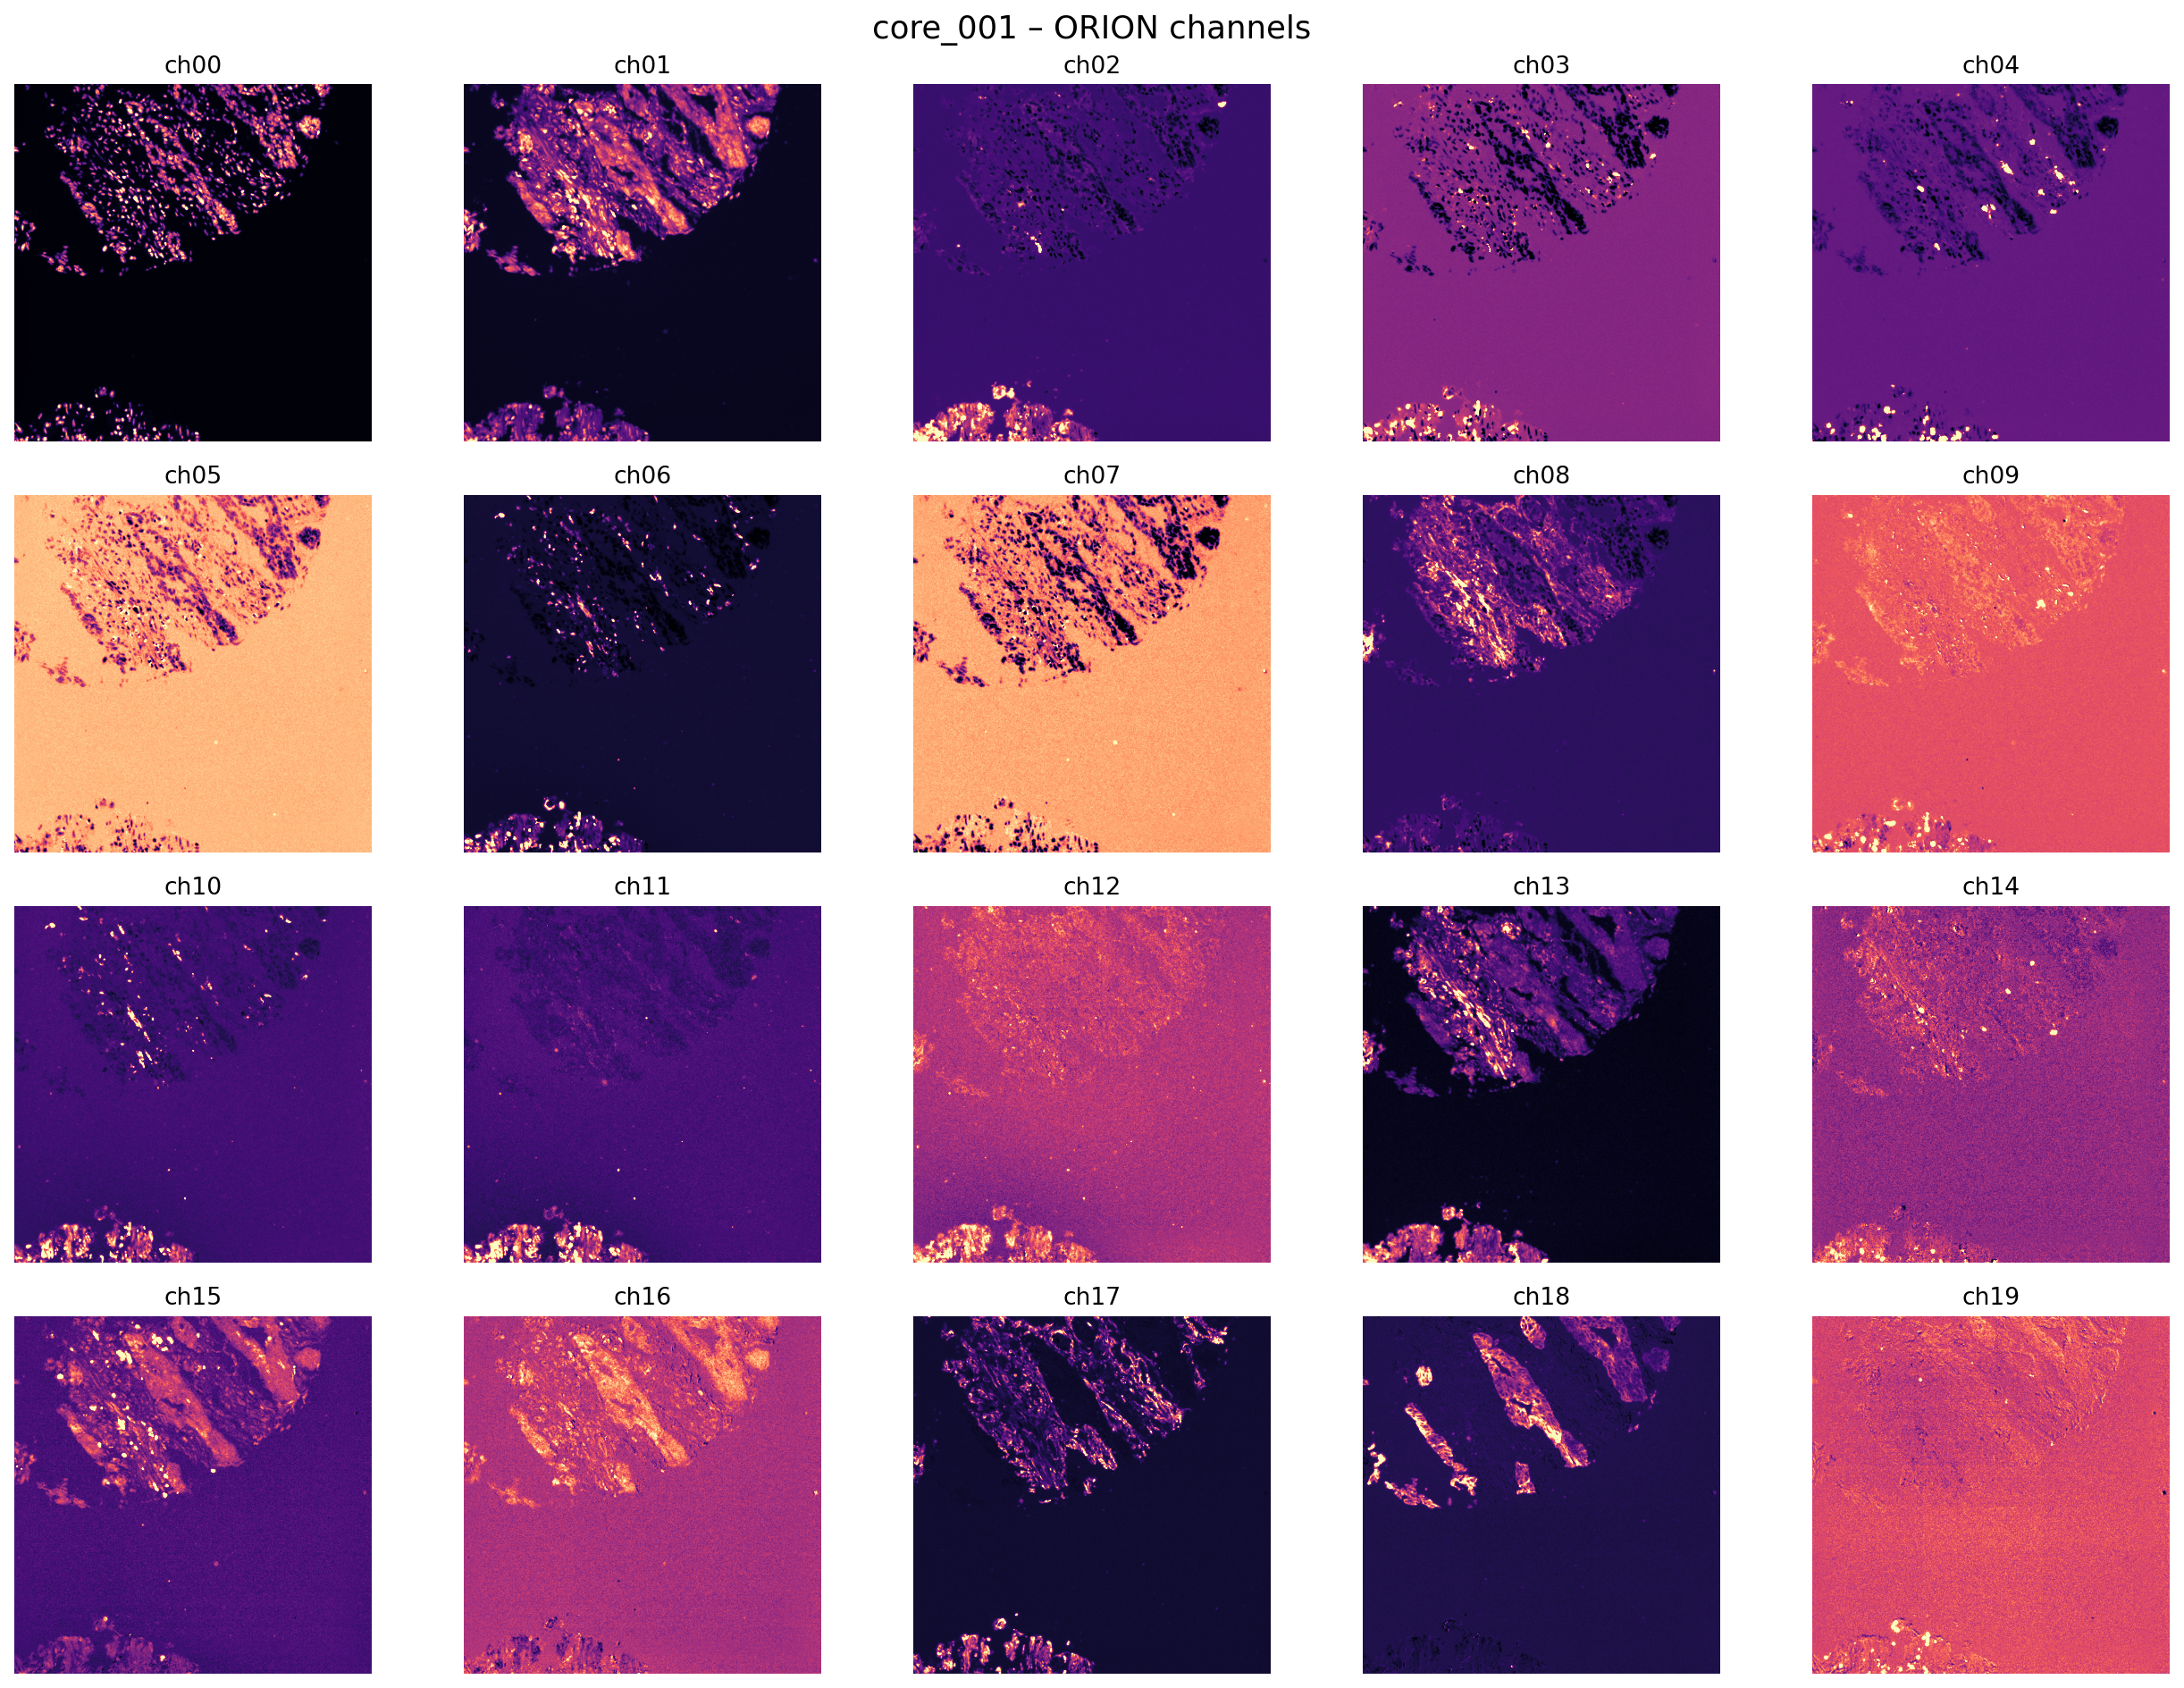
\includegraphics[width=\textwidth]{../output/visualize_nov4/core_001_orion_channels.png}\\[4pt]
      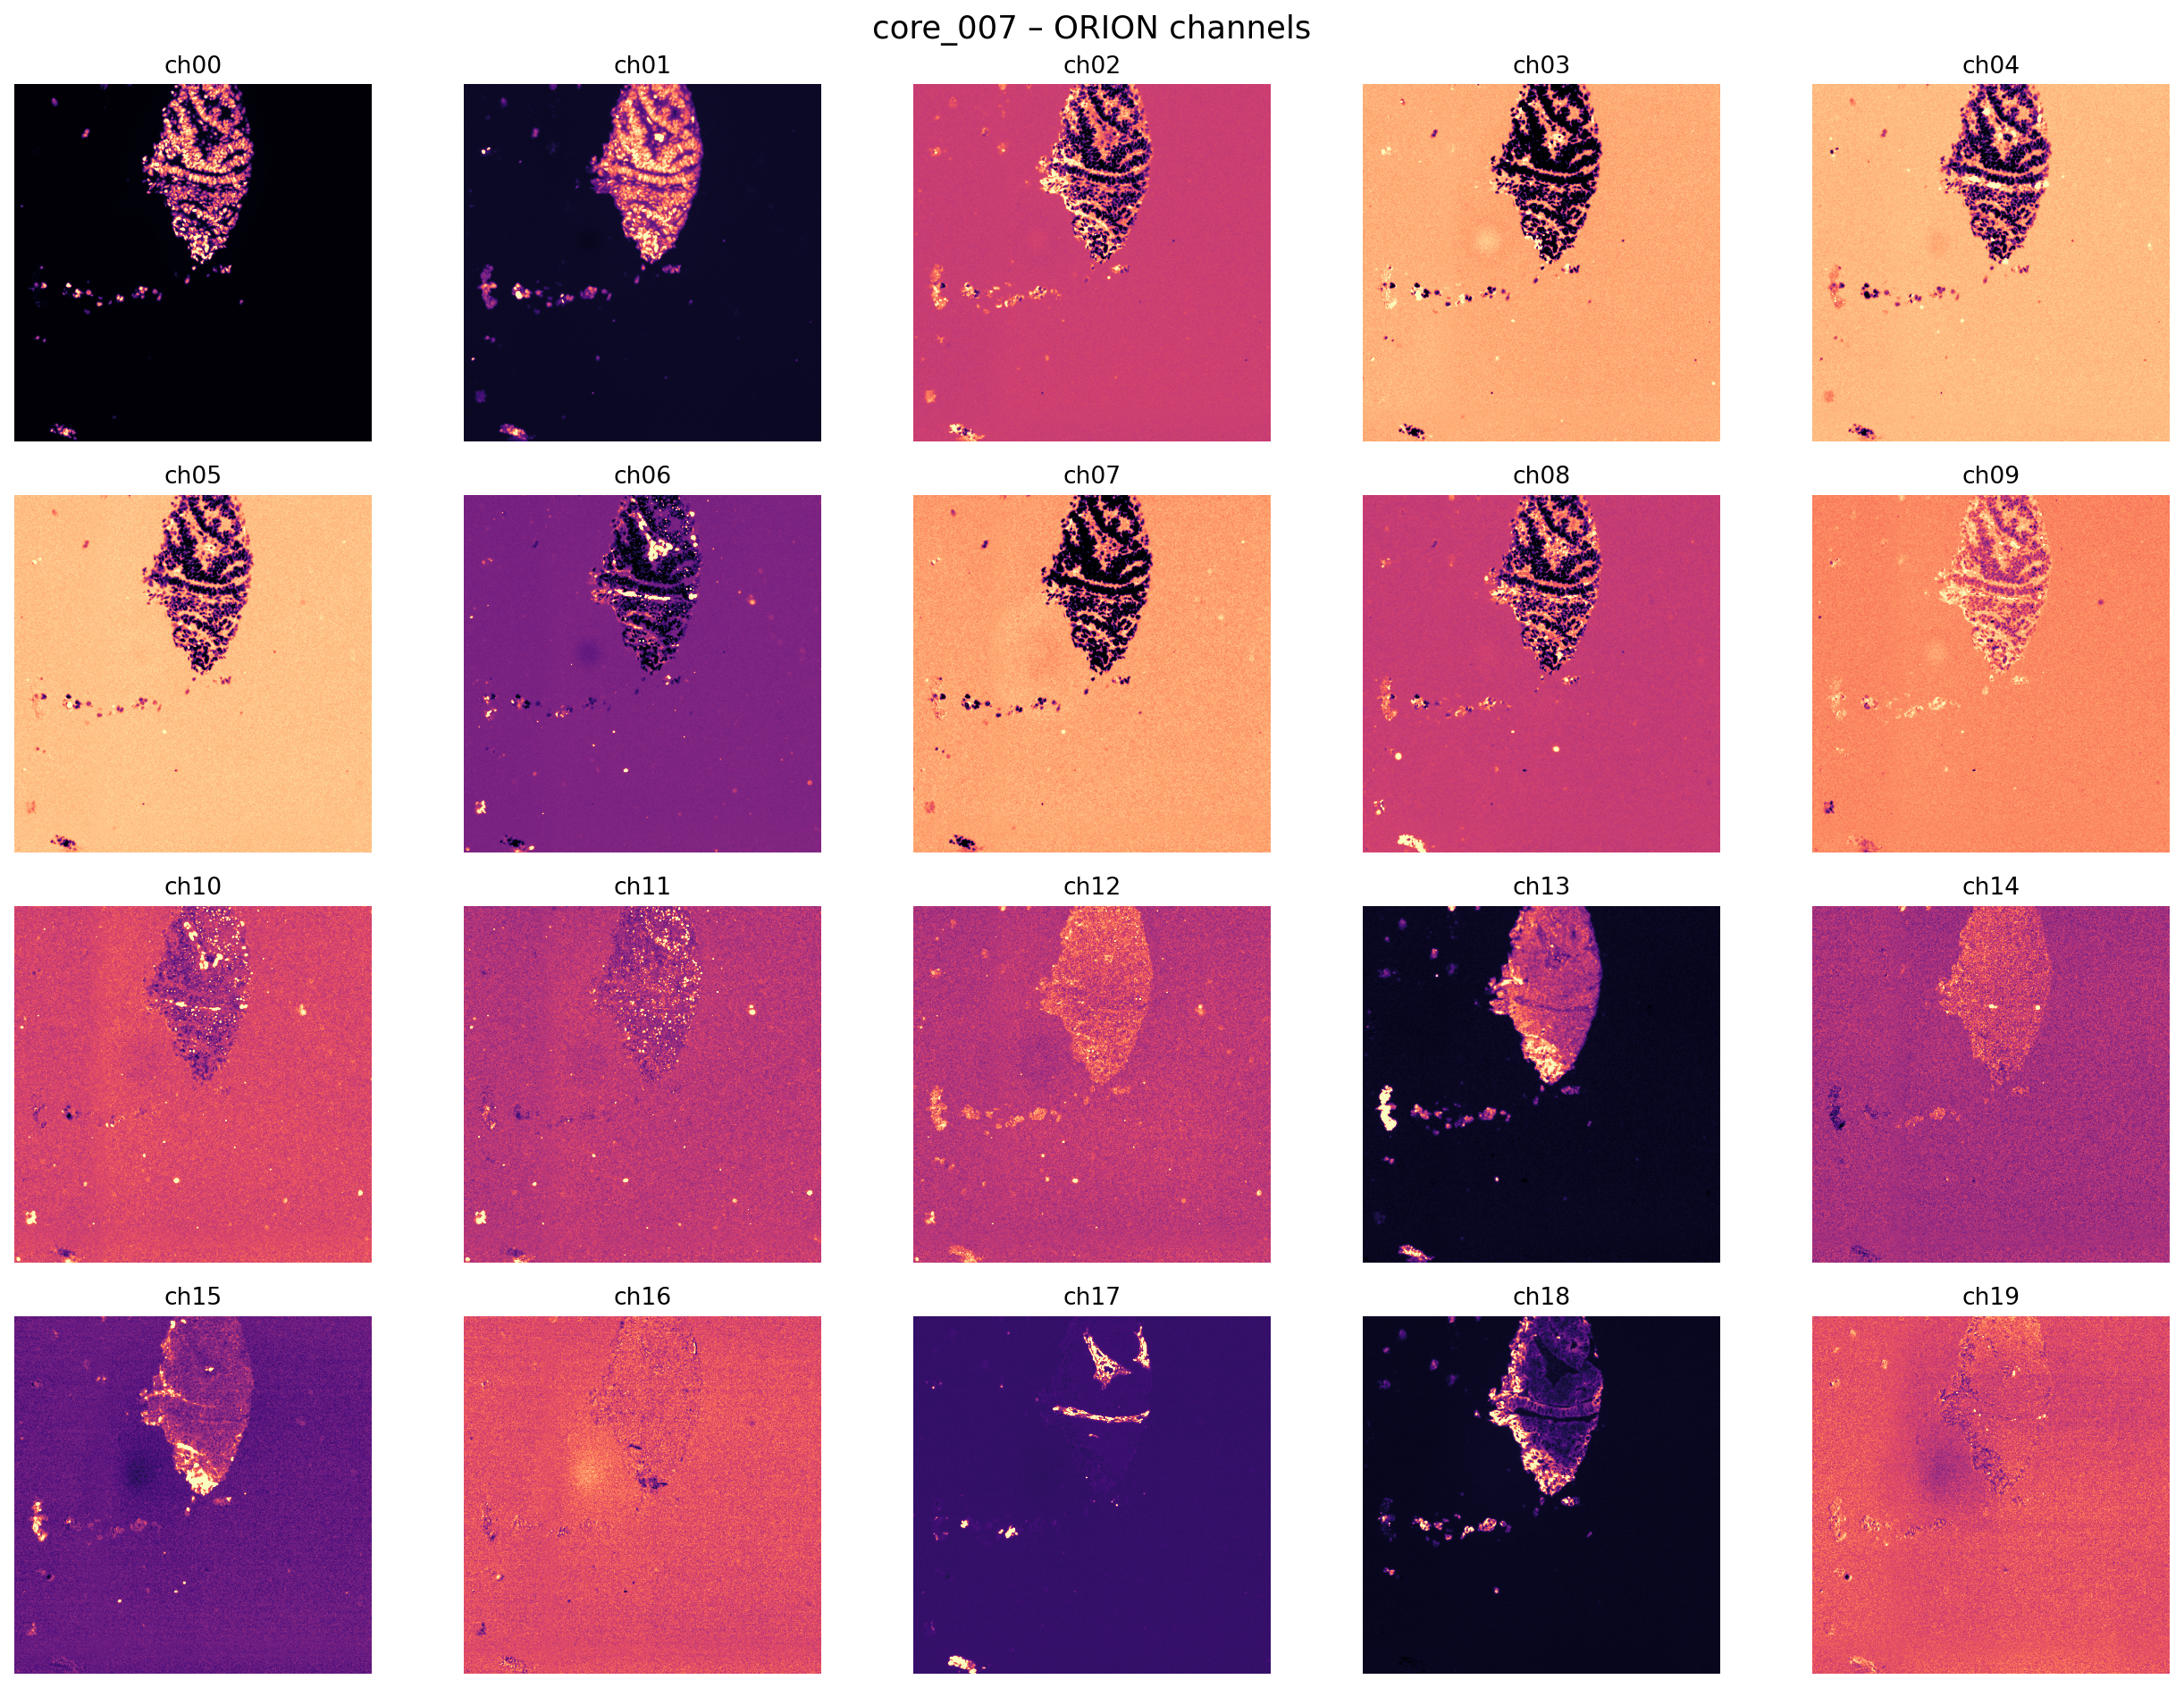
\includegraphics[width=\textwidth]{../output/visualize_nov4/core_007_orion_channels.png}
    \end{column}
  \end{columns}
\end{frame}

\begin{frame}{Extended QC Gallery}
  \begin{columns}[T]
    \begin{column}{0.48\textwidth}
      \includegraphics[width=\textwidth]{../output/visualize_nov4/core_073_he.png}\\[4pt]
      \includegraphics[width=\textwidth]{../output/visualize_nov4/core_272_he.png}
    \end{column}
    \begin{column}{0.48\textwidth}
      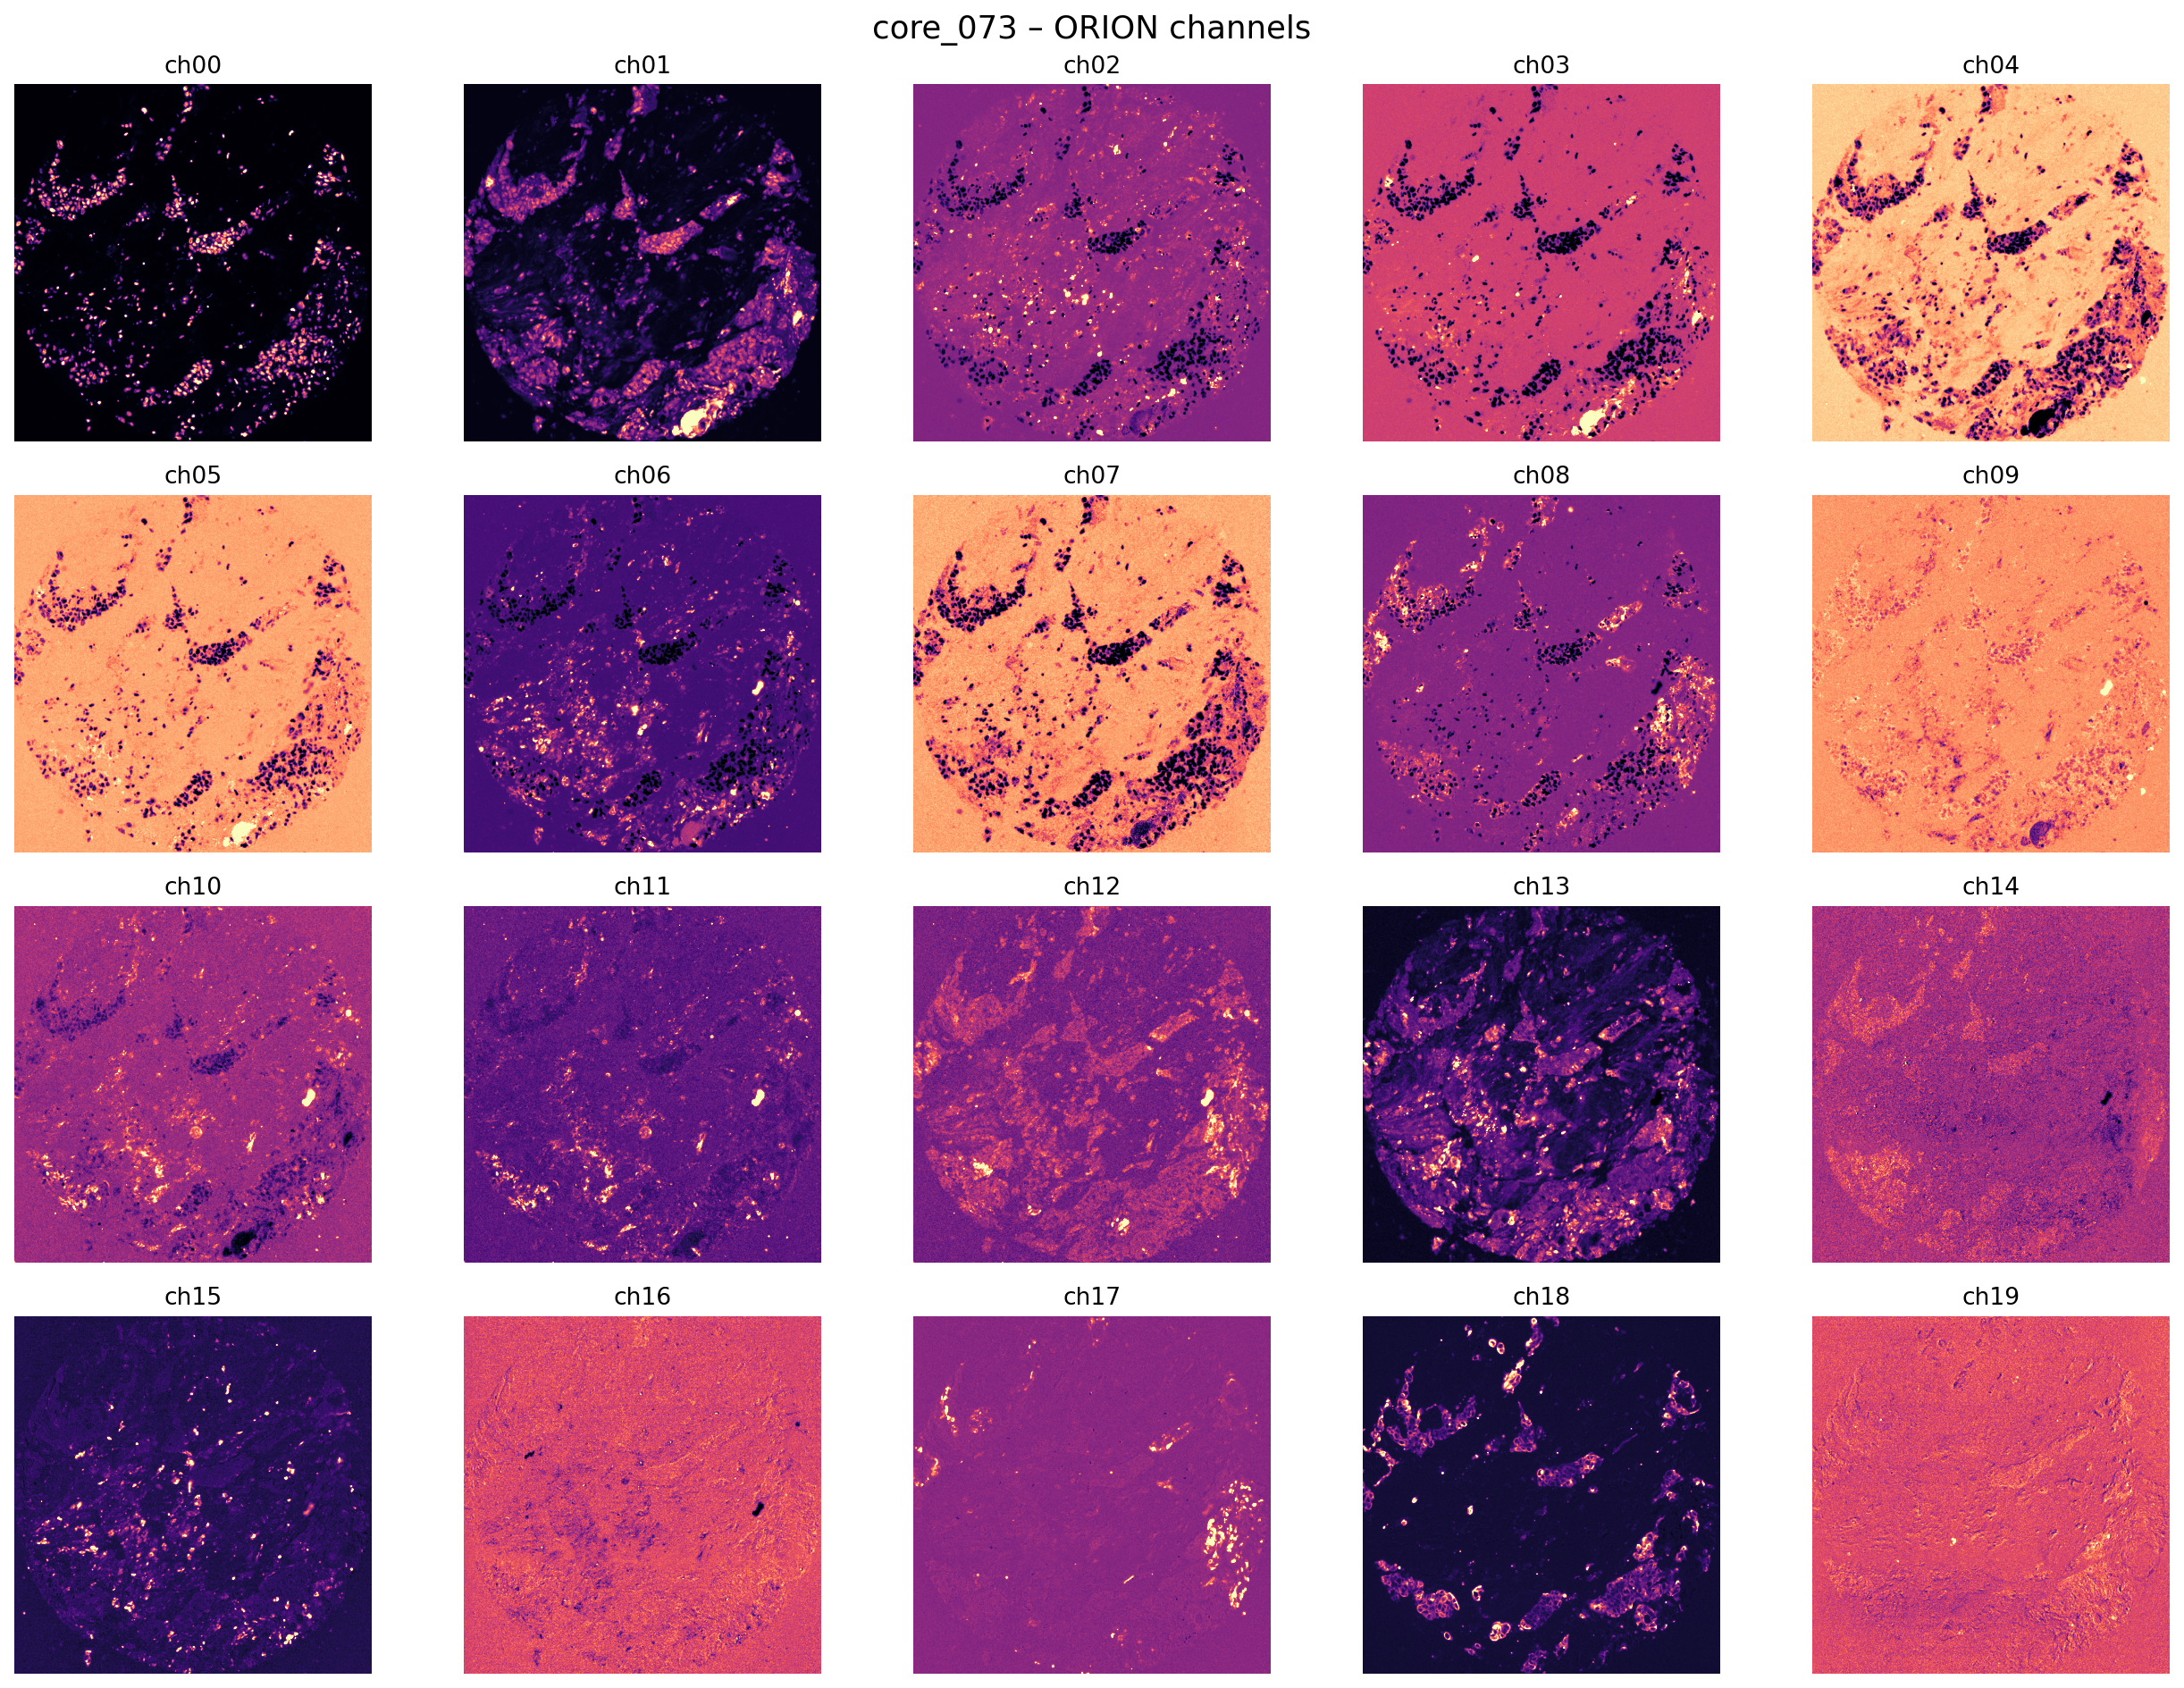
\includegraphics[width=\textwidth]{../output/visualize_nov4/core_073_orion_channels.png}\\[4pt]
      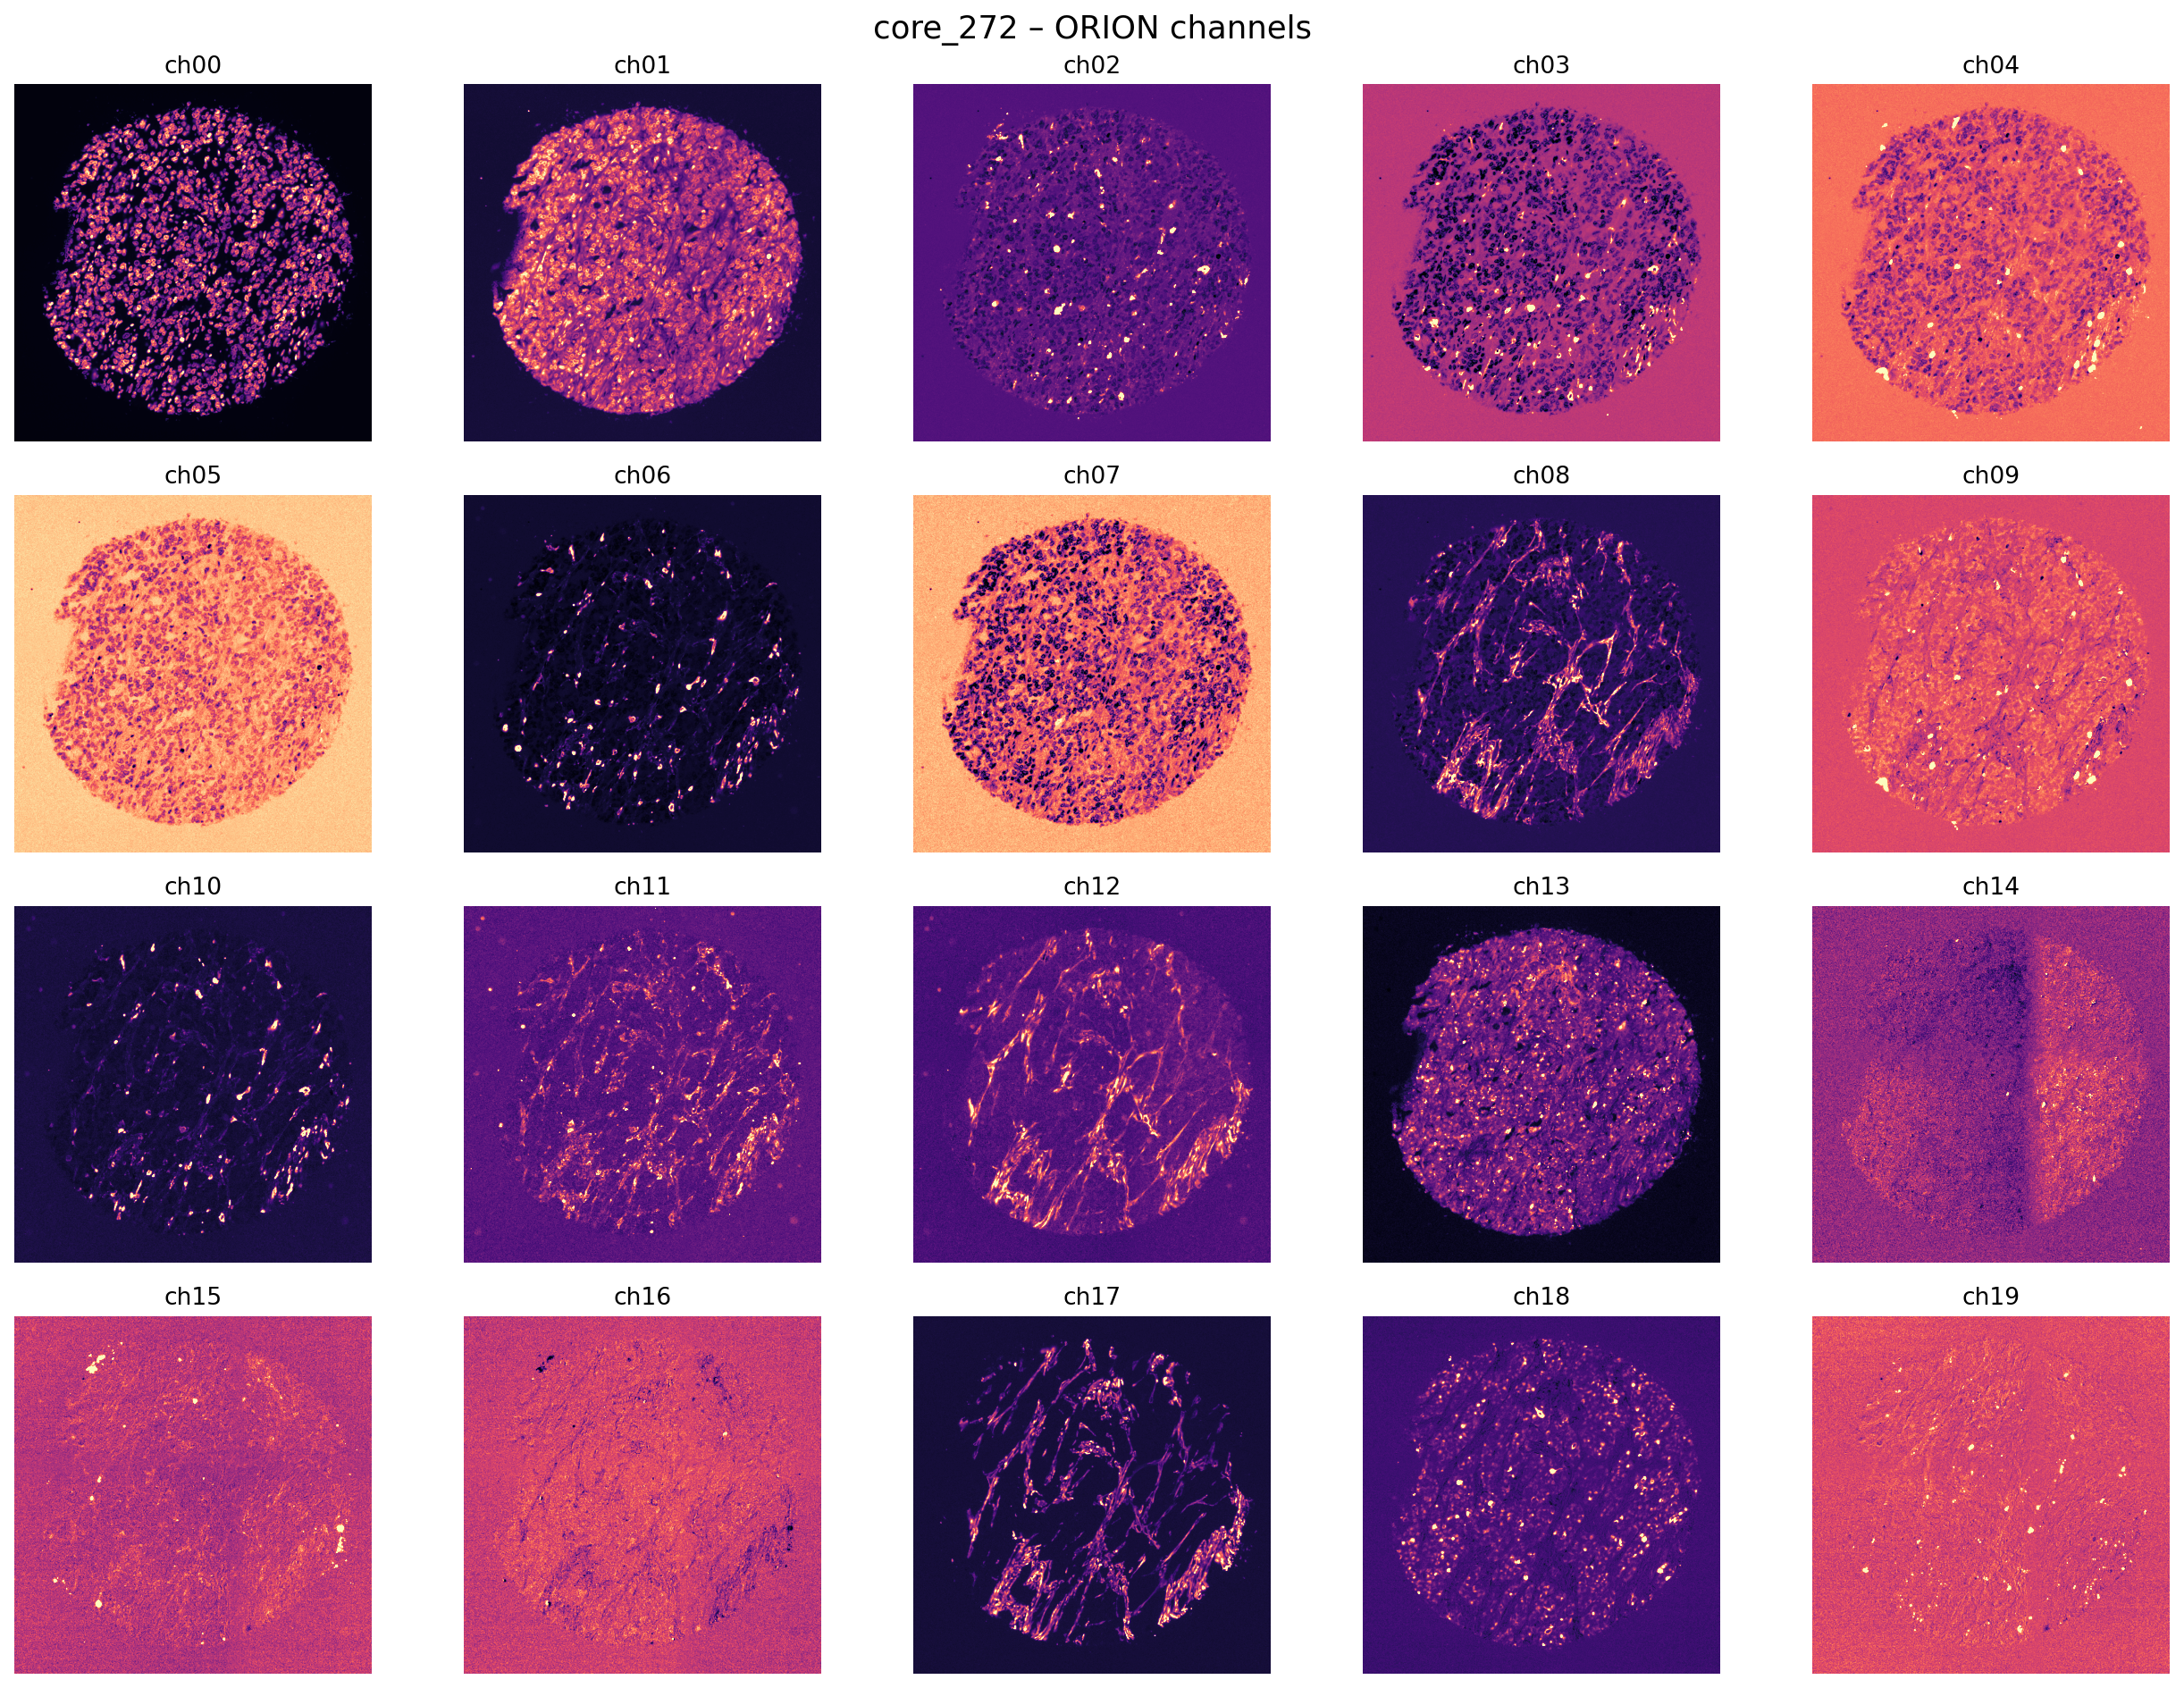
\includegraphics[width=\textwidth]{../output/visualize_nov4/core_272_orion_channels.png}
    \end{column}
  \end{columns}
\end{frame}

\begin{frame}{Model vs Ground Truth Placeholders}
  \begin{columns}[T]
    \begin{column}{0.48\textwidth}
      \fbox{\parbox{\textwidth}{\centering INSERT SWIN-UNET vs GT (core\_001)\\per-channel montage}}
    \end{column}
    \begin{column}{0.48\textwidth}
      \fbox{\parbox{\textwidth}{\centering INSERT CONVNEXT vs GT (core\_001)\\per-channel montage}}
    \end{column}
  \end{columns}
  \vspace{1em}
  \centering
  \fbox{\parbox{0.85\textwidth}{\centering INSERT CHANNEL TRIPTYCH (FOLR2 / CD163 / SPP1)}}
\end{frame}

\begin{frame}{Comparative Observations}
  \begin{itemize}
    \item Swin-UNet maintains morphology on sparse macrophage markers; reduced halo artefacts.
    \item ConvNeXt-UNet sharper on abundant epithelial markers (Pan-CK, SMA) but noisier on low coverage.
    \item Channel-aware sampling benefits both; evaluate cross-site generalisation in next phase.
    \item Future: ensemble or knowledge distillation to balance accuracy vs efficiency.
  \end{itemize}
\end{frame}

\begin{frame}{Novelty vs Literature}
  \begin{itemize}
    \item Full 20-channel Orion prediction with global quantile scaling and speckle-aware sampling.
    \item Presence-aware auxiliary head uncommon in prior H\&E $\rightarrow$ IF translation studies.
    \item End-to-end pipeline: registration, QC, DDP training for large cohorts.
    \item Extends beyond prior single-marker virtual staining and GAN-based approaches.
  \end{itemize}
\end{frame}

\begin{frame}{Related Work}
  \begin{itemize}
    \item Rivenson et al., \emph{PNAS} 2019: Virtual staining of auto-fluorescence (single channel).
    \item Fu et al., \emph{Nat. Biomed. Eng.} 2020: Hyperspectral marker imputation without channel-aware sampling.
    \item Lu et al., \emph{Med. Image Anal.} 2022: GAN-based H\&E $\rightarrow$ IF translation, limited scaling.
  \end{itemize}
  \vspace{0.5em}
  \centering
  \fbox{\parbox{0.85\textwidth}{\centering ADDITIONAL REFERENCES / DOI LINKS AS NEEDED}}
\end{frame}

\begin{frame}{Pathologist-Focused Takeaways}
  \begin{itemize}
    \item Rapid in silico multiplexing to prioritise cores for lab validation.
    \item Channel coverage maps and presence logits offer interpretability hooks.
    \item Feedback requested: critical markers, acceptable error ranges, integration needs.
  \end{itemize}
\end{frame}

\begin{frame}{Next Steps}
  \begin{itemize}
    \item Export quantitative metrics (PSNR/SSIM per channel); align with human review.
    \item Automate registration QA alerts for misaligned cores.
    \item Extend to additional TA cohorts; collect clinical endpoints for outcome modelling.
    \item Investigate uncertainty estimates and active learning for rare marker discovery.
  \end{itemize}
\end{frame}

\begin{frame}{Discussion}
  \centering
  \Large Questions, feedback, and marker priorities welcome.
\end{frame}

\end{document}

